\documentclass{article}

\usepackage{listings}
\usepackage{hyperref}
\usepackage{pdfpages}
\usepackage{commons/course}
\usepackage{authoraftertitle}
\usepackage{graphicx}
\usepackage[dvipsnames]{xcolor}
\usepackage{booktabs} % To thicken table lines

\newcommand\myshade{85}
\colorlet{mylinkcolor}{violet}
\colorlet{mycitecolor}{violet}
\colorlet{myurlcolor}{violet}

\hypersetup{
	linkcolor  = mylinkcolor!\myshade!black,
	citecolor  = mycitecolor!\myshade!black,
	urlcolor   = myurlcolor!\myshade!black,
	colorlinks = true,
}


\definecolor{codegreen}{rgb}{0,0.6,0}
\definecolor{codegray}{rgb}{0.5,0.5,0.5}
\definecolor{codepurple}{rgb}{0.58,0,0.82}
\definecolor{backcolour}{rgb}{0.95,0.95,0.92}


\lstdefinestyle{mystyle}{
    backgroundcolor=\color{backcolour},   
    commentstyle=\color{codegreen},
    keywordstyle=\color{magenta},
    numberstyle=\tiny\color{codegray},
    stringstyle=\color{codepurple},
    basicstyle=\ttfamily\footnotesize,
    breakatwhitespace=false,         
    breaklines=true,                 
    captionpos=b,
    keepspaces=true,                 
    numbers=left,                    
    numbersep=5pt,                  
    showspaces=false,                
    showstringspaces=false,
    showtabs=false,                  
    tabsize=2
}

\lstset{style=mystyle}

\author{
نیم‌سال دوم ۹۹-۰۰
}
\title{
تمرین سری چهارم
}
\date{\today}

\begin{document}

\heading{\MyTitle}{}{شبکه‌های عصبی}{\MyAuthor}

\section*{تشخیص ارقام دست‌نویس}

در این تمرین، می‌خواهیم به کمک شبکه‌های عصبی مسئلهٔ
\lr{classification}
تصویر ارقام دست‌نویس را حل کنیم. مجموعه داده‌های مورد استفاده در این مسئله، برگرفته از مجموعه داده‌های
\hyperref{http://yann.lecun.com/exdb/mnist/}{}{}{\lr{MNIST}}
است که برای این تمرین، اندکی مورد پردازش قرار گرفته است. چند نمونه از تصاویر این مجموعه داده در شکل
\ref{fig:MNIST}
نشان داده شده‌است. این مجموعه داده شامل ۹۸۰۰۰ تصویر ۲۸ در ۲۸ برای آموزش شبکه (با برچسب) و ۲۱۰۰۰ تصویر (بدون برچسب) برای ارزیابی مدل و نمره‌دهی است.

\begin{figure}[ht]
\begin{center}
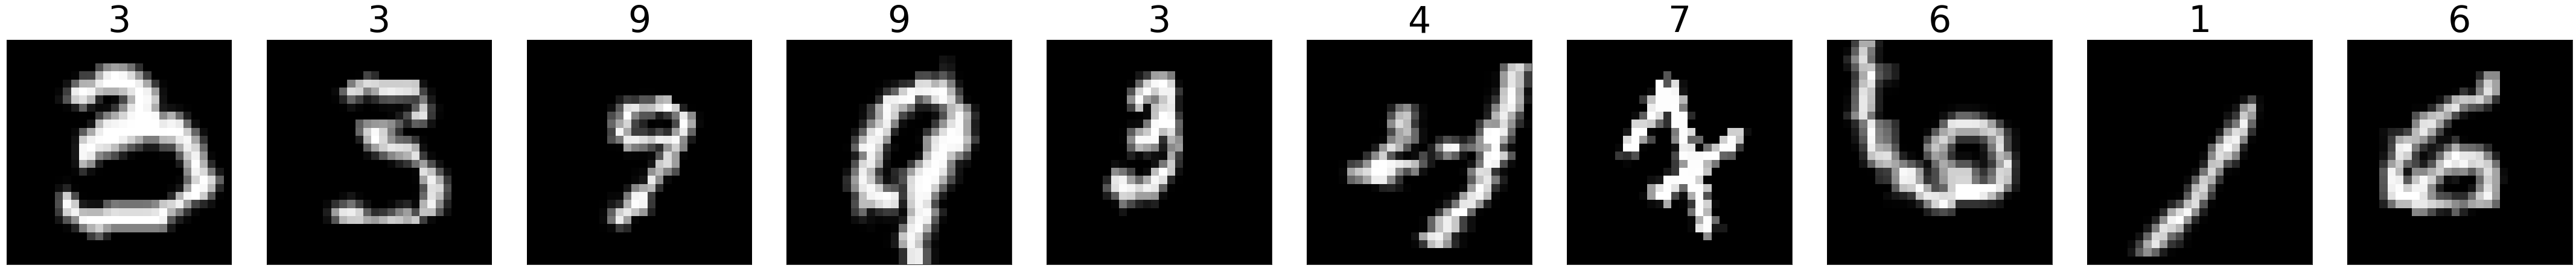
\includegraphics[width=\linewidth]{images/figure.png}
\caption{چند نمونه از تصاویر مجموعه دادهٔ مسئله}
\label{fig:MNIST}
\end{center}
\end{figure}

به همراه این فایل، یک فایل جوپیتر نوت‌بوک نیز در اختیارتان قرار گرفته است که بایستی پیاده‌سازی و آموزش شبکه عصبی خود را در آن انجام دهید. آن چه تحویل خواهید داد، فایل نوت‌بوک مذکور و فایل
\lr{prediction}
داده‌های ارزیابی است. فایل
\lr{hw4\_helper.py}
نیز حاوی توابع کمکی برای دریافت دیتاست و ذخیره
\lr{prediction}
است که در ادامه نحوه استفاده از آن شرح داده شده‌است.

\subsection*{دریافت داده‌ها}

برای دریافت داده‌ها می‌توانید از توابع زیر استفاده کنید:

\begin{latin}
\begin{lstlisting}[language=Python]
import hw4_helper
x_train, y_train = hw4_helper.get_train_data()
x_test = hw4_helper.get_test_data()
\end{lstlisting}
\end{latin}

این توابع، برای اولین بار فایل دیتاست را دانلود کرده و در فولدر
\lr{data\_cache}
ذخیره می‌کنند. در دفعات بعدی چون فایل‌ها در آن مسیر موجود اند، تصاویر بدون دانلود مجدد از همان‌جا
\lr{load}
می‌شوند. در صورت بروز هرگونه مشکل با توابع مذکور، می‌توانید فایل
\hyperref{https://drive.google.com/file/d/1-0iZwp7vygQqXNLaDmORp_d_EDQVrBXz/view?usp=sharing}{}{}{\lr{x\_train}}،
\hyperref{https://drive.google.com/file/d/1-4be9NCtS_fhFePJP1T_92iAhwCvwGuQ/view?usp=sharing}{}{}{\lr{y\_train}}
و
\hyperref{https://drive.google.com/file/d/1-4A5ZY2jdOFKnupZ2eBB2P4EJI-4im7p/view?usp=sharing}{}{}{\lr{x\_test}}
را دانلود کرده و با استفاده از تابع
\lr{np.load('path/to/file')}
آن‌ها را
\lr{load}
کنید.

\textbf{نکته مهم:}
برای آموزش شبکه خود فقط و فقط از
\lr{x\_train}
و
\lr{y\_train}
استفاده کنید.

\subsection*{طراحی مدل}

پیشنهاد می‌شود برای طراحی مدل خود، از کتابخانه‌های
\hyperref{https://pytorch.org/}{}{}{\lr{PyTorch}}،
\hyperref{https://www.tensorflow.org/}{}{}{\lr{Tensorflow}}
یا
\hyperref{https://keras.io/}{}{}{\lr{Keras}}
استفاده کنید. مدل شما باید یک
\lr{batch}
از تصاویر را که ابعاد آن
$B \times 28 \times 28$
است را دریافت کرده و به ازای هر تصویر، یک بردار ۱۰ بعدی بعنوان خروجی برگرداند که هر عنصر آن، احتمال هریک از برچسب‌ها (ارقام ۰ تا ۹) باشد. (ابعاد خروجی باید
$B \times 10$
باشد.)

ساده‌ترین مدلی که می‌توانید طراحی کنید، فقط شامل لایه‌های
\hyperref{https://pytorch.org/docs/stable/generated/torch.nn.Linear.html}{}{}{\lr{Fully Connected}}
است. در این حالت، باید تصاویر خود را بصورت یک آرایهٔ یک‌بعدی (با
$28 \times 28 = 784$
عنصر) به مدل بدهید. در مدل نیز کافیست بصورت پشت سر هم، لایه‌های خطی را با تابع فعال‌سازی
\hyperref{https://pytorch.org/docs/stable/generated/torch.nn.ReLU.html}{}{}{\lr{ReLU}}
قرار دهید. در آخرین لایه (که شامل ۱۰ نورون است) نیز باید از تابع فعال‌سازی
\hyperref{https://pytorch.org/docs/stable/generated/torch.nn.Softmax.html}{}{}{\lr{Softmax}}
استفاده کنید. این تابع مجموع خروجی‌های هر نمونه را برابر ۱ قرار می‌دهد تا بتوان به هر یک از عناصر آن بعنوان احتمال نگاه کرد.

با استفاده از شبکه‌های
\lr{Fully Connected}
می‌توانید به دقت مورد انتظار برای دریافت نمره کامل در این مسئله برسید. اما برای دقت‌های بالاتر و دریافت نمره امتیازی، بهتر است از شبکه‌های عصبی کانولوشنی استفاده کنید. برای این کار، ابتدا توسط لابه‌های
\hyperdef{https://pytorch.org/docs/stable/generated/torch.nn.Conv2d.html}{}{}{کانولوشنی دوبعدی}
و تابع فعال‌سازی
\lr{ReLU}،
ابعاد تصویر را کاهش، و تعداد کانال‌های آن را افزایش دهید. (برای کاهش ابعاد تصاویر، هم می‌توانید از لایه‌ی کانولوشنی با
\lr{stride}
برابر ۲ استفاده کنید، هم می‌توانید از لایه‌های
\lr{Pooling}
مثل
\hyperref{https://pytorch.org/docs/stable/generated/torch.nn.MaxPool2d.html}{}{}{\lr{Max Pooling}}
استفاده کنید.) پس از کاهش ابعاد تصاویر و افزایش کانال‌های آن به اندازه کافی، آن را بصورت یک‌بعدی در آورده و توسط یک شبکهٔ
\lr{Fully Connected}،
مشابه چیزی که بالاتر شرح داده شد خروجی را تولید کنید.

همچنین برای جلوگیری از
\lr{overfitting}،
می‌توانید از لایه‌های
\lr{Dropout}
و
\lr{Batch Normalization}
در میان لایه‌های شبکه خود استفاده کنید. در
\hyperref{https://pytorch.org/tutorials/beginner/blitz/cifar10_tutorial.html}{}{define-a-convolutional-neural-network}{این لینک}،
می‌توانید یک پیاده‌سازی بسیار ساده از یک شبکه عصبی کانولوشنی در کتابخانه
\lr{PyTorch}
را مشاهده کنید.

\subsection*{تابع هزینه و روش بهینه‌سازی}

برای مسئلهٔ
\lr{classification}
چند کلاسه، عموماً از تابع هزینهٔ
\hyperref{https://pytorch.org/docs/master/generated/torch.nn.functional.cross_entropy.html}{}{}{\lr{cross-entropy}}
استفاده می‌شود. روش‌های بهینه‌سازی متنوعی نیز قابل استفاده اند، که از جمله آن‌ها می‌توان به
\hyperref{https://pytorch.org/docs/master/generated/torch.optim.Adam.html}{}{}{\lr{Adam}}
و
\hyperref{https://pytorch.org/docs/master/generated/torch.optim.SGD.html}{}{}{\lr{SGD}}
اشاره کرد.

\subsection*{آموزش شبکه}

برای آموزش شبکه خود، بخش کوچکی از داده‌های آموزشی (مثلاً ۱۰ درصد) را برای اعتبارسنجی
(\lr{validation})
در نظر بگیرید. (می‌توانید از
\hyperref{https://scikit-learn.org/stable/modules/generated/sklearn.model_selection.train_test_split.html}{}{}{این}
تابع استفاده کنید.) سپس در هر
\lr{epoch}،
داده‌های آموزشی را به تعدادی
\lr{batch}
تقسیم کرده، و هر یک را به مدل دهید. با استفاده از تابع هزینه، هزینهٔ خروجی محاسبه شده را بدست آورید و با استفاده از روش بهینه‌سازی، وزن‌های مدل خود را به‌روزرسانی کنید. علاوه بر محاسبهٔ هزینهٔ مجموع هر
\lr{epoch}،
دقت (نسبت تعداد تشخیص‌های درست به کل تصاویر) را نیز محاسبه کرده و در یک لیست ذخیره کنید.

در هر
\lr{epoch}
پس از آموزش شبکه، هزینه و دقت را روی داده‌های اعتبارسنجی نیز انجام دهید و نتایج را ذخیره کنید. توجه کنید که در اعتبارسنجی، به هیچ وجه از بهینه‌سازی استفاده نکنید.

\subsection*{رسم نمودار آموزش شبکه}

مطابق شکل
\ref{fig:TrainingCurve}،
نمودارهای روند پیش‌روی هزینه و دقت مدل روی داده‌های آموزشی و اعتبارسنجی مدل را رسم کنید.

\begin{figure}[ht]
	\begin{center}
		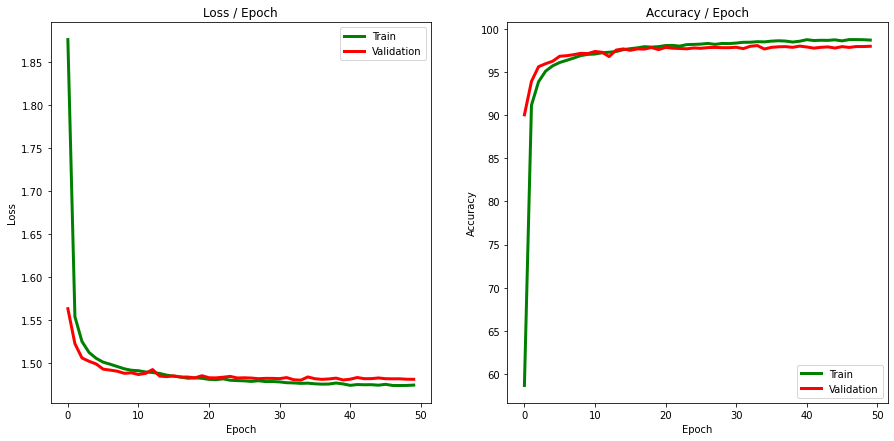
\includegraphics[width=\linewidth]{images/TrainingCurve.png}
		\label{fig:TrainingCurve}
		\caption{نمودار آموزش شبکه}
	\end{center}
\end{figure}


\subsection*{اجرای مدل روی داده‌های تست و ذخیره خروجی آن در فایل}

در نهایت، مدل با کمترین هزینه اعتبارسنجی را انتخاب کرده، و خروجی آن به ازای داده‌های تست بدست آورید. خروجی احتمال را با استفاده از تابع
\lr{argmax}
به برچسب تبدیل کنید. (به ازای هر نمونه،‌ یک عدد بین ۰ تا ۹ به آن نسبت دهید.) سپس بردار یک‌بعدی حاصل را با استفاده از تابع زیر ذخیره کنید.

\begin{latin}
\begin{lstlisting}[language=Python]
hw4_helper.export_prediction(prediction)
\end{lstlisting}
\end{latin}

این تابع، فایل 
\lr{prediction.npy}
را در کنار نوت‌بوک می‌سازد. این فایل را به همراه نوت‌بوک نهایی به فرمت
\lr{zip}
در آورده و در کوئرا بارگذاری کنید.

\end{document}